\section{Benchmark NIST-7 "Boundary Line Singularity"}
\label{sec:bench-7}

This is a singularity problem with a solution that is singular along the left boundary.
The equation of this problem is Poisson equation

\begin{equation} \label{boundary-line-singularity}
-\Delta u = f
\end{equation}
in the domain $\Omega = (0, 1)^2$, equipped with Dirichlet boundary conditions
given by the exact solution.

The exact solution
\begin{equation}\label{exact-nist-7}
u(x,y) = x^{\alpha}
\end{equation}
where $\alpha \geq 0.5$ determines the strength of the singularity.
The right-hand side $f$ is calculated by inserting (\ref{exact-nist-7}) into (\ref{boundary-line-singularity}).
The solution of NIST-7 with $\alpha = 0.6$ is shown in Fig. \ref{fig:sln-nist07}.

\begin{figure}[!ht]
\centering
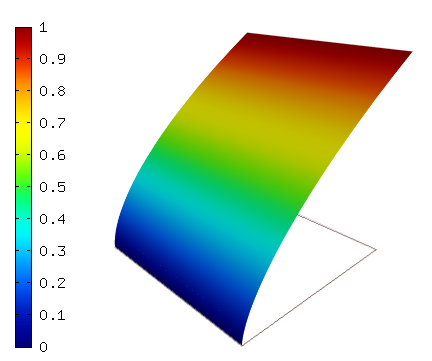
\includegraphics[height=6cm]{nist/nist-7/solution.png}
\caption{The solution to NIST-7 benchmark problem.}
\label{fig:sln-nist07}
\end{figure}
